%
% main.tex -- Paper zum Thema <mongekant>
%
% (c) 2020 Autor, OST Ostschweizer Fachhochschule
%
% !TEX root = ../../buch.tex
% !TEX spellcheck = de_CH
% !TEX encoding = UTF-8
%
\newcommand{\wasserstein}[1][p]{\mathcal{W}_{#1}}
\chapter{Optimaler Transport\label{chapter:mongekant}}
\kopflinks{Optimaler Transport}
\begin{refsection}
\chapterauthor{Patrik Müller}

\noindent
Wie transportiere ich eine Ladung effizient von A nach B?
Diese Frage beschäftigt die Menschheit seit jeher --
vom Umlagern von Getreidekörnern auf dem Feld
bis zum Versenden von Paketen in globalen Logistiknetzen.

Im 18.~Jahrhundert stellte der französische Mathematiker Gaspard Monge
im Dienste Napoléon Bonapartes genau dieselbe Frage:
Wie kann man Erde von einem Ort zum anderen bewegen,
um eine Befestigung zu errichten,
sodass die dafür notwendige Arbeit minimal ist?
1781 veröffentlichte er ein präzises mathematisches Modell,
das heute als Monge‑Problem des optimalen Transports bekannt ist.

Im 20.~Jahrhundert erweiterte Leonid Witaljewitch~Kantorowitch das Modell,
indem er einige von Monge aufgestellte Forderungen lockerte.
Diese Relaxation führt zur linearen Optimierungsformulierung,
die heute als Kantorowitch‑Problem bezeichnet wird
und den Grundstein für die moderne Theorie des optimalen Transports legt.
Für diesen bahnbrechenden Beitrag erhielt Kantorowitch 1975
den Nobelpreis für Wirtschaftswissenschaften.

In diesem Kapitel werden beide Modelle vorgestellt und miteinander verglichen.
Zudem werden einige Anwendungen des optimalen Transports diskutiert.

In diesem Kapitel stellen wir zunächst beide Modelle vor,
erläutern ihre mathematischen Grundlagen, sowie Eigenschaften und
stellen einen Verbindung zur Feldtheorie her.
Anschliessend diskutieren wir ausgewählte Anwendungen des optimalen Transports
aus unterschiedlichen Bereichen.


%
% einleitung.tex -- Beispiel-File für die Einleitung
%
% (c) 2020 Prof Dr Andreas Müller, Hochschule Rapperswil
%
% !TEX root = ../../buch.tex
% !TEX encoding = UTF-8
%
\section{Mathematisches Grundgerüst\label{mongekant:section:teil0}}
\kopfrechts{Mathematisches Grundgerüst}

Um die Modelle des optimalen Transports zu verstehen,
müssen wir uns zunächst mit einigen mathematischen Grundlagen vertraut machen.
Damit die Konzepte klar werden,
werden wir die Theorie anhand eines anschaulichen Beispiels mit Sandhaufen erläutern.

\subsection{Transport von Masse\label{mongekant:subection:transport}}
Stellen wir uns vor,
wir wollen einen Sandhaufen im Raum $X$
in einen neuen Sandhaufen im Raum $Y$ transportieren.
Eine Teilmenge $A\subset X$ des Quellhaufens enthält die Masse $\mu(A)$,
was man sich als die Masse einer Schaufel Sand vorstellen kann.
Analog enthält eine Teilmenge $B\subset Y$ des Zielhaufens die Masse $\nu(B)$.

Der Transport wird durch eine Abbildung
\begin{align*}
T\colon X\to Y
,\qquad y=T(x)
\end{align*}
beschrieben,
die jedem Punkt $x\in X$ einen Zielpunkt $y\in Y$ zuordnet.
Damit die Masse beim Transport erhalten bleibt,
muss für jede messbare Teilmenge $B\subset Y$
\begin{align*}
\nu(B)
&=
\mu(A)
\\
&=
\mu\left(T^{-1}(B)\right)
=
T_{\#}\mu(B)
\end{align*}
gelten.
$T_{\#}\mu$ wird in der Literatur als \emph{Push-Forward} von $\mu$ nach $\nu$ durch $T$ bezeichnet.
In Abbildung~\ref{mongekant:fig:optimal_transport} ist der 1-dimensionale Fall dargestellt.

\begin{figure}
\centering
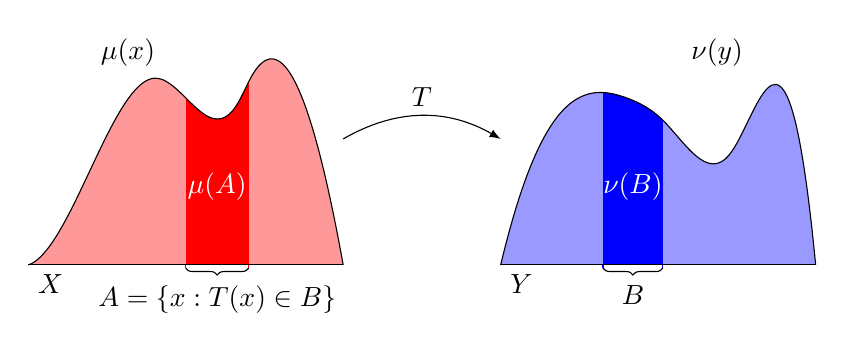
\begin{tikzpicture}[>=latex]
  % Define some colors for consistency
  \def\intensity{0.6}
  \definecolor{lightblue}{rgb}{\intensity, \intensity, 1}
  \definecolor{lightred}{rgb}{1, \intensity, \intensity}
  \def\pathA{(0.000, 0.000) .. controls (0.169, 0.054) and (0.338, 0.507) .. (0.507, 0.837)
   .. controls (0.606, 1.032) and (0.706, 1.184) .. (0.806, 1.186)
   .. controls (0.980, 1.189) and (1.154, 0.733) .. (1.328, 1.022)
   .. controls (1.359, 1.073) and (1.390, 1.147) .. (1.420, 1.201)
   .. controls (1.536, 1.402) and (1.651, 1.317) .. (1.766, 0.989)
   .. controls (1.844, 0.766) and (1.922, 0.432) .. (2.000, 0.000)}
  \def\pathB{(0.000, 0.000) .. controls (0.123, 0.515) and (0.246, 0.802) .. (0.368, 0.951)
   .. controls (0.518, 1.133) and (0.667, 1.112) .. (0.817, 1.054)
   .. controls (0.883, 1.028) and (0.948, 0.995) .. (1.014, 0.934)
   .. controls (1.161, 0.797) and (1.309, 0.516) .. (1.456, 0.705)
   .. controls (1.598, 0.886) and (1.740, 1.503) .. (1.882, 0.862)
   .. controls (1.921, 0.684) and (1.961, 0.408) .. (2.000, 0.000)}
  \def\Astart{1.0}
  \def\Aend{1.4}
  \def\Bstart{0.65}
  \def\Bend{1.03}
  \def\tickheight{0.02}
  \def\drawscale{2}
  \def\xlast{2cm}
  \def\boffset{\drawscale*3cm}
  \def\arrowoffset{0.8cm}

  % Left Blob (Initial Distribution)
  \begin{scope}[scale=\drawscale,red]
    \fill[lightred] \pathA;
    \begin{scope}
      \clip \pathA;
      \fill (\Astart, 0.0) rectangle (\Aend, 1.5);
    \end{scope}
    \draw[black] \pathA;
    \draw (\Astart, 0) -- (\Astart, -\tickheight) coordinate (A_start_tick);
    \draw (\Aend, 0) -- (\Aend, -\tickheight) coordinate (A_end_tick);
    \draw[black,decorate,decoration={brace,mirror}] (A_start_tick) -- (A_end_tick)
      node[midway,below=0.1cm] {$A = \left\{ x : T(x) \in B \right\}$};
    \node[anchor=north west,color=black] at (0.2*\xlast, 1.5cm) {$\mu(x)$};
    \node[anchor=center,color=white] at (0.5*\Astart + 0.5*\Aend, 0.5cm) {$\mu(A)$};
    \draw[black] (0,0) node [black,below right]{$X$} -- (\xlast,0);
  \end{scope}

  % Right Blob (Transformed Distribution)
  \begin{scope}[xshift=\boffset,scale=\drawscale,anchor=south west,color=blue]
    \fill[lightblue] \pathB;
    \begin{scope}
      \clip \pathB;
      \fill (\Bstart, 0.0) rectangle (\Bend, 1.5);
    \end{scope}
    \draw[black] \pathB;
    \draw (\Bstart, 0) -- (\Bstart, -\tickheight) coordinate (B_start_tick);
    \draw (\Bend, 0) -- (\Bend, -\tickheight) coordinate (B_end_tick);
    \draw[black,decorate,decoration={brace,mirror}] (B_start_tick) -- (B_end_tick)
      node[midway,below=0.1cm] {$B$};
    \node[anchor=north east,color=black] at (0.8*\xlast, 1.5cm) {$\nu(y)$};
    \node[anchor=center,color=white] at (0.5*\Bstart + 0.5*\Bend, 0.5cm) {$\nu(B)$};
    \draw[black] (0,0) node [black,below right]{$Y$} -- (\xlast,0);
  \end{scope}

  \draw[->, bend angle=30] (\drawscale*\xlast, \drawscale * \arrowoffset) to [bend left]
    node[above]{$T$} (\boffset, \drawscale * (\arrowoffset);

  % % Arrow
  % \draw[->, very thick] (6,0) to [bend right=30] (0,0);
  % \node at (3, 0.8) {$T$};
  %
  % % Labels for distributions
  % \node at (-1, -1) {$dv = \rho(q) dq$};
  % \node at (7, -1) {$du = \rho(x,t) dx$};
\end{tikzpicture}

\caption{1-dimensionaler Transport von $\mu(A)$ nach $\nu(B)$ mittels Abbildung $T$}
\label{mongekant:fig:optimal_transport}
\end{figure}

In vielen Anwendungen sind $\mu$ und $\nu$ Wahrscheinlichkeitsmasse,
also gilt
\begin{align*}
\mu(X)
&=
\nu(Y)
=
1
.
\end{align*}
Befindet sich $\mu$ (bzw. $\nu$) im absolut stetigen Fall,
existieren Dichten $f,g\in L^{1}$ mit
\begin{align}
\begin{aligned}
\mu(A)
&=
\int_A f(x) \, dx
\\
\nu(B)
&=
\int_B g(y) \, dy
.
\end{aligned}
\label{mongekant:eq:absolute_continuity}
\end{align}

\subsection{Kosten des Transports\label{mongekant:subsection:transport_cost}}
Nun stellt sich die Frage,
wie \glqq teuer\grqq{} der Transport von $A$ nach $B$ ist.
Dazu führen wir eine Kostenfunktion $c : X \times Y \to [0, +\infty]$ ein,
die die Kosten $c(x,y)$ für den Transport eines Sandkorns
von $x \in X$ nach $y \in Y$ angibt.
Die Gesamtkosten $I$ für den Transport $T$ von $X$ nach $Y$ sind dann
\begin{align}
I(T)
&=
\int_X c\,\Bigl(x, T(x)\Bigr) \, d\mu(x)
\label{mongekant:eq:monge_transport_cost}
.
\end{align}
Die Schreibweise $d\mu(x)$ ist die übliche Formulierung des
Lebesgue‑Integrals über ein beliebiges Mass.
Man kann sich $d\mu(x)$ als \glqq infinitesimale Masse\grqq{} vorstellen,
die an der Stelle $x$ liegt.
Oder um unsere Sandhaufen-Analogie vorzusetzen,
die Masse eines einzelnen Sandkorns.
In der Literatur wird auch oft die alternative Schreibweise $\mu(dx)$ verwendet,
diese suggeriert jedoch fälschlicherweise dass die Masse unabhängig vom Ort ist,
was im Allgemeinen nicht der Fall ist.
Deshalb benutzen wir ausschliesslich die Schreibweise $d\mu(x)$.

%
% teil1.tex -- Beispiel-File für das Paper
%
% (c) 2020 Prof Dr Andreas Müller, Hochschule Rapperswil
%
% !TEX root = ../../buch.tex
% !TEX encoding = UTF-8
%
\section{Monge-Formulierung%
\label{mongekant:section:teil1}}
\kopfrechts{Monge-Formulierung}

Nachdem die Grundbegriffe des Transports eingeführt wurden,
formulieren wir das von Gaspard Monge (1781) aufgestellte Optimierungsproblem.
Dazu können wir \eqref{mongekant:eq:monge_transport_cost} verwenden,
um die günstigsten Transportkosten zu berechnen:
\begin{align}
C_M(\mu, \nu)
&:=
\inf_{T}
\int_X c\,\Bigl(x, T(x)\Bigr)\, d\mu(x)
,\quad
\text{wobei } T_{\#}\mu=\nu
.
\label{mongekant:eq:monge_problem}
\end{align}
Wir verwenden das \emph{Infimum} und nicht das \emph{Minimum},
weil es nicht immer eine Abbildung $T$ gibt,
die das Infimum annimmt.
Ein konkretes Gegenbeispiel sehen wir in
Abschnitt~\ref{mongekant:subsection:monge_inexistence}.

\subsection{Spezialfälle mit Existenzgarantie}
Zwei besonders wichtige Fälle,
in denen das Infimum tatsächlich ein Minimum ist,
sind:
\begin{itemize}
\item Der diskreten Fall, wenn
\begin{align*}
\mu
&=
\frac{1}{n} \sum_{i=1}^n \delta_{x_i}
\\
\nu
&=
\frac{1}{n} \sum_{j=1}^n \delta_{y_j}
,
\end{align*}
wobei $\delta$ die Dirac-Funktion bezeichnet.
\item Der absolut stetigen Fall, wenn
\begin{align}
\begin{aligned}
d\mu
&=
f(x)\, dx
\\
d\nu
&=
g(y)\, dy
.
\end{aligned}
\label{mongekant:eq:absolute_densities}
\end{align}
Diesen Zusammenhang erhält man,
wenn man \eqref{mongekant:eq:absolute_continuity} ableitet und
Gleichheit für alle möglichen Teilmengen $A$ und $B$ fordert.
\end{itemize}
Die Beweise für die Existenz eines optimalen Transports $T$ in beiden Szenarien
benötigen tiefere Resultate aus Topologie und Masstheorie und
liegen ausserhalb des Umfangs dieses Seminars.

\subsection{Zusammenhang mit der Monge-Ampère-Gleichung}
Der interessierte Leser fragt sich vielleicht,
ob die Monge-Ampère-Gleichung~\eqref{mongeampere:eq:mongeampere}
aus Kapitel~\ref{chapter:mongeampere}
mit dem Monge-Problem zusammenhängt.
Tatsächlich gibt es einen Zusammenhang,
den wir nun kurz erläutern wollen.

Betrachten wir den absolut stetigen Fall aus \eqref{mongekant:eq:absolute_densities}.
Wir wissen,
dass die Massenerhaltung gilt,
also muss
\begin{align*}
\int_{A} f(x) \, dx
&=
\int_{T(A)} g(y) \, dy
\end{align*}
für alle messbaren $A$ gelten.
Setzt man $y = T(x)$,
folgt
\begin{align*}
\int_{A} f(x) \, dx
&=
\int_{A} g\,\Bigl(T(x)\Bigr) \det\Bigl(DT(x)\Bigr) \, dx
.
\end{align*}
Wird nun $T = \nabla \varphi$ gewählt,
wobei $\varphi$ eine konvexe Funktion ist,
die zweimal stetig differenzierbar ist,
ergibt sich
\begin{align*}
\int_{A} f(x) \, dx
&=
\int_{T(A)} g\,\Bigl(\nabla \varphi(x)\Bigr) \det\Bigl(D^2 \varphi(x)\Bigr) \, dx
.
\end{align*}
Da die Gleichheit für alle messbaren $A$ gelten muss,
kann man die Integranden gleichsetzen und erhält
\begin{align*}
f(x)
&=
g\,\Bigl(\nabla \varphi(x)\Bigr) \det\Bigl(D^2 \varphi(x)\Bigr)
.
\end{align*}
Löst man nach $\det(D^2 \varphi(x))$ auf,
folgt die Monge-Ampère-Gleichung
\begin{align*}
\det\,\Bigl(D^2 \varphi(x)\Bigr)
&=
\frac{f(x)}{g\,\Bigl(\nabla \varphi(x)\Bigr)}
.
\end{align*}
In \cite{mongekant:brenier} wird eindrücklich gezeigt,
dass die Abbildung $T = \nabla \varphi$
die eindeutige Lösung des Monge-Problems \eqref{mongekant:eq:monge_problem} ist,
wenn $c(x,y) = \left\lvert x - y\right\rvert^2$ ist und die obigen Bedingungen gelten.

\subsection{Fallbeispiel: Nichtexistenz einer Lösung%
\label{mongekant:subsection:monge_inexistence}}
Betrachten wir den Fall,
in dem die Quellverteilung $\mu$ eine Punktmasse an Stelle $x_1$ ist,
\begin{align*}
\mu
&=
\delta_{x_1}
\end{align*}
und die Zielverteilung $\nu$ aus zwei unterschiedlichen Punkten besteht
\begin{align*}
\nu
&=
\frac{1}{2} \delta_{y_1} + \frac{1}{2} \delta_{y_2}
,\quad
\text{wobei } y_1 \neq y_2
.
\end{align*}
Dann gilt $\nu(\{y_1\}) = \frac{1}{2}$,
aber für
\begin{align*}
\mu\left(\left\{T^{-1}(y_1)\right\}\right)
=
\begin{cases}
0,
&\text{wenn }
T^{-1}(y_1)
\neq
x_1
\\
1,
&\text{wenn }
T^{-1}(y_1)
=
x_1
.
\end{cases}
\end{align*}
Somit kann kein Bildmass $T_{\#}\mu$ die Gleichung $T_{\#}\mu=\nu$ erfüllen --
das Monge‑Problem \eqref{mongekant:eq:monge_problem}
besitzt in diesem Beispiel keine Lösung.



%
% teil2.tex -- Beispiel-File für teil2
%
% (c) 2020 Prof Dr Andreas Müller, Hochschule Rapperswil
%
% !TEX root = ../../buch.tex
% !TEX encoding = UTF-8
%
\section{Teilweise Reflexion, Transmission und Absorption an einer Grenzfläche
\label{schall:section:teil2}}
\kopfrechts{Teil 2}

In diesem Abschnitt untersuchen wir eine ebene, zeit\-harmonische Schallwelle,
die aus Medium~1 auf eine ebene Grenzfläche zu Medium~2 trifft.
Ein Teil der Welle wird reflektiert, ein Teil wird transmittiert.
Im einfachsten Fall vernachlässigbarer Verluste, genügen die Druck- und
Geschwindigkeitsfelder in beiden Medien der linearen Akustik;
bei realen Medien müssen Absorption, Transmission und Reflexion ebenfalls
berücksichtigt werden.
Diese können durch einen komplexen Wellenzahl- oder Impedanzterm
ermittelt werden, was in diesem Abschnitt beschrieben wird.
\todo[inline]{Grafik: Grenzfläche mit einfallender, reflektierter und transmittierter Welle}

\subsection{Randbedingungen und Definitionen (Normal\-einfall)}
Wir betrachten eine ebene Welle, die senkrecht auf die Grenzfläche trifft.
Die Druckanteile lauten
\[
    p_i(x,t)=\Re( P_i\,e^{\mathrm{i}(\omega t-k_1 x)}),\quad
    p_r(x,t)=\Re( P_r\,e^{\mathrm{i}(\omega t+k_1 x)}),\quad
    p_t(x,t)=\Re( P_t\,e^{\mathrm{i}(\omega t-k_2 x)}),
\]
wobei die Indexschreibweise $i,r,t$ für \emph{incident}, \emph{reflected} und \emph{transmitted} steht.
Die charakteristische akustische Impedanz sei für Fluide $Z_n=\rho_n c_n$, $n\in\{1,2\}$.
An der Grenzfläche $x=0$ fordern wir Kontinuität von Druck und Normalgeschwindigkeit:
\[
    p_i+p_r=p_t,\qquad \frac{p_i-p_r}{Z_1}=\frac{p_t}{Z_2}.
\]
Daraus folgen die \emph{amplitudenbezogenen} Reflexions- und Transmissionskoeffizienten
\begin{equation}
    R_p=\frac{P_r}{P_i}=\frac{Z_2-Z_1}{Z_2+Z_1},
    \qquad
    T_p=\frac{P_t}{P_i}=\frac{2Z_2}{Z_2+Z_1}.
    \label{eq:RpTp}
\end{equation}
Für Intensitäten, sprich für den Leistungsfluss, ergibt sich bei reellen Impedanzen \cite{schall:kinsler, schall:allenRT}
\begin{equation}
    R_I=\left|R_p\right|^2=\left(\frac{Z_2-Z_1}{Z_2+Z_1}\right)^2,\qquad
    T_I=\frac{4Z_1Z_2}{(Z_2+Z_1)^2},
    \qquad
    R_I+T_I=1.
    \label{eq:RI_TI}
\end{equation}
\todo[inline]{Umfomuleren}

\subsection{Absorption im zweiten Medium}
Reale Medien weisen Dämpfung auf, sprich es kommt zu einer
verlustbehafteten Transmission.
Dies lässt sich mit einem \emph{komplexen Wellenzahl}
\(
    k_2 = \beta_2 - \mathrm{i}\alpha
\)
oder äquivalent mit einer \emph{komplexen Impedanz} modellieren.
Für die \emph{Amplitude} des transmittierten Drucks gilt entlang $x>0$
\[
    |P_t(x)| = |P_t(0)|\,e^{-\alpha x},
\]
woraus für die \emph{Intensität} die Exponentialabnahme
\begin{equation}
    I_t(x)=I_i\,T_I\,e^{-2\alpha x}
    \label{eq:intensity_decay}
\end{equation}
bei ebenen Wellen folgt.
Für viele Medien wird die frequenzabhängige Dämpfung durch ein Gesetz
$\alpha(\omega)=\alpha_0\,\omega^\eta$ beschrieben
(Materialklassen: $\eta\in[0,2]$) \cite{schall:allenAbsorption}.

Damit definiert man die \emph{absorptionsbezogene Energiebilanz} über einer Strecke $L$ in Medium~2:
\begin{equation}
    1 \;=\; R_I \;+\; T_I\,e^{-2\alpha L} \;+\; A(L),
    \qquad
    A(L)=1-R_I - T_I e^{-2\alpha L},
    \label{eq:absorption_balance}
\end{equation}
wobei $A(L)$ der bis zur Tiefe $L$ absorbierte Intensitätsanteil ist.
Im Spezialfall einer \emph{dünnen, rein absorbierenden Schicht},
sprich ein Dämpfungs\-modell ohne Mehrfachreflexionen, geht
$A \approx 1-R_I-T_I$ für $L\to0$ über.
Experimentell wird die \emph{Absorptionskoeffizient}
$\alpha_\mathrm{surf}$ häufig über Impedanz\- bzw.\ Stehwellen\-rohre
bestimmt; für Normal\-einfall gilt (aus dem gemessenen Stehwellenverhältnis SWR)
\begin{equation}
    \alpha_\mathrm{surf} \;=\; 1 - R_I \;=\; 1 - \left(\frac{\mathrm{SWR}-1}{\mathrm{SWR}+1}\right)^2,
    \label{eq:alpha_SWR}
\end{equation}
wobei
\[
    \mathrm{SWR} = \frac{p_\mathrm{max}}{p_\mathrm{min}} = \frac{1+|R_p|}{1-|R_p|}
\]
das Stehwellenverhältnis ist.

\paragraph{Bemerkung zu komplexen Impedanzen.}
Sind Materialverluste in $Z_2$ als $Z_2(\omega)\in\mathbb{C}$ erfasst,
bleiben \eqref{eq:RpTp} formal gültig; für Intensitäten ist dann
\[
    R_I=\left|R_p\right|^2,\qquad
    T_I=\frac{4\,\Re\{Z_1\}\,\Re\{Z_2\}}{|Z_1+Z_2|^2},
\]
wobei $Z_1$ für Fluide typischerweise reell ist.
In vielen Anwendungen ist die Modellierung über $k_2=\beta_2-\mathrm{i}\alpha$
mittels \eqref{eq:intensity_decay} praktischer \cite{schall:kinsler,schall:allenRT}.

\subsection{Schräg\-einfall}
Für Schräg\-einfall gilt die akustische Snell'sche Brechung
\(
    \sin\theta_1/c_1=\sin\theta_2/c_2
\),
und die \emph{normale} Impedanzkomponente skaliert zu
$Z_{n} = Z/\cos\theta$ (Fluid--Fluid).
Entsprechend ändern sich $R_p$, $T_p$ und damit $R_I$, $T_I$;
jenseits des kritischen Winkels tritt ein evaneszentes Feld in
Medium~2 auf, dessen Amplitude exponentiell abnimmt.
Ein evaneszentes Feld ist eine scheinbare, sich nicht ausbreitende
im zweiten Medium, die nicht als laufende Welle in die Tiefe propagiert,
sondern exponentiell zur Grenzfläche hin abklingt \cite{schall:wikiSnell}.
\todo[inline]{Herleitung}
%
% teil3.tex -- Beispiel-File für Teil 3
%
% (c) 2020 Prof Dr Andreas Müller, Hochschule Rapperswil
%
% !TEX root = ../../buch.tex
% !TEX encoding = UTF-8
%
\section{Schallausbreitung bei Überschallflugzeugen
\label{schall:section:teil3}}
\kopfrechts{Teil 3}

In diesem Abschnitt wenden wir die in den vorherigen Abschnitten
beschriebenen Konzepte an, um die Schallausbreitung bei einem
Flugzeug im Überschall zu beschreiben.
Dabei betrachten wir eine ideale Situation, in der das Flugzeug als
Punktquelle modelliert wird.

Wir betrachten ein Flugzeug, das sich mit konstanter Geschwindigkeit
$V>0$ entlang einer horizontalen Bahn auf der Höhe $z=z_a$ über
dem Grund $z=0$ bewegt.
Das Medium sei ein ideales Gas mit örtlich variabler Temperatur
$T(z)$ aber ohne Wind, sodass
\begin{equation}
    c(z) \;=\; \sqrt{\kappa R_S\,T(z)} ,
    \label{eq:c-of-z}
\end{equation}
gilt. Hier ist $c(z)$ die lokale Schallgeschwindigkeit, $R_S = \frac{R}{M}$
die Massenangepasste Gaskonstante und $M$ die auf der Höhe $z$ herrschende
molare Masse des Mediums.
In der Fliegerei wird die Geschwindigkeit des Flugzeugs oft über die
dimensionslose \emph{Machzahl} $Ma$ angegeben:
\begin{equation}
    Ma(z) \;=\; \frac{V}{c(z)},
    \label{eq:mach-number}
\end{equation}
wobei $Ma<1$ Unterschall, $Ma=1$ Schallgeschwindigkeit und $Ma>1$ Überschall
bezeichnet.
Der Effekt des Schall- oder Machkegels, welcher durch den Dopplereffekt
beschrieben wird, ist im Bild \ref{fig:schall:mach-zones} visualisiert.

\begin{figure}
    \centering
    \includegraphics[width=\textwidth]{papers/schall/figures/mach_doppler_triptych_offsets.png}
    \caption{Dopplereffekt bei Unterschall, Schallgeschwindigkeit und Überschall.
    Für die Schallgeschwindigkeit und den Überschall ist zusätzlich der
    Machkegel mit dem Machwinkel $\mu$ eingezeichnet.}
    \label{fig:schall:mach-zones}
\end{figure}

\subsection{Lokaler Machwinkel und Emissionsrichtung}
In einem homogenem Medium bildet sich der Machkegel mit Halbwinkel
\begin{equation}
    \mu \;=\; \arcsin\!\Big(\frac{1}{Ma}\Big).
\end{equation}
In einem geschichteten Medium setzt man diesen \emph{lokal} an der
Emissionshöhe $z_a$, auf welcher das Flugzeug fliegt, an:
\begin{equation}
    \mu_a \;:=\; \arcsin\!\Big(\frac{1}{Ma(z_a)}\Big)
    \;=\; \arcsin\!\Big(\frac{c(z_a)}{V}\Big) .
    \label{eq:local-mach-angle}
\end{equation}
Der Rand des Machkegels wird oft als Machrand bezeichnet, welcher im
vertikalen Schnitt $(x,z)$ durch akustische Strahlen begrenz ist.
Dies nennt man die \emph{geometrische Akustik}.

\subsection{Strahlen in geschichtetem Medium}
Für isotrope, ruhende Medien mit $c=c(z)$ liefert die geometrische
Akustik eine Snell-ähnliche Invariante:
\begin{equation}
    \frac{\sin\theta(z)}{c(z)} \;=\; \text{const} \;=:\; K ,
    \label{eq:snell-acoustics}
\end{equation}
wobei $\theta(z)$ der Winkel des Strahls relativ zur Horizontalen ist.
Wählt man als Anfangsbedingung den lokalen Machwinkel an $z=z_a$,
also $\theta(z_a)=\mu_a$, dann folgt aus \eqref{eq:snell-acoustics}
\[
    K \;=\; \frac{\sin\mu_a}{c(z_a)} \;=\; \frac{1/M(z_a)}{c(z_a)} \;=\; \frac{1}{V}.
\]
Damit ist für Mach-Strahlen die Invariante schlicht
\begin{equation}
    K \;=\; \frac{1}{V}.
    \label{eq:K-equals-1-over-V}
\end{equation}

Mit $\tan\theta = \dfrac{dz}{dx}$, $\sin\theta = K\,c(z)$ und
$\cos\theta = \sqrt{1 - \sin^2\theta}$,
erhält man nach der Trigonometrie
\begin{equation}
    \frac{dz}{dx} \;=\; \frac{\sin\theta(z)}{\cos\theta(z)} \;=\;
    \frac{K\,c(z)}{\sqrt{1 - K^2 c^2(z)}}.
\end{equation}
Einsetzen von \eqref{eq:K-equals-1-over-V} liefert die
\emph{Bahn-Differentialgleichung} der Mach-Ränder:
\begin{equation}
    \quad
    \frac{dz}{dx} \;=\; \frac{c(z)/V}{\sqrt{1 - \big(c(z)/V\big)^2}}
    \;=\; \frac{1}{\sqrt{\frac{V^2}{c^2(z)} - 1}}
    \quad
    \label{eq:ray-ode}
\end{equation}
oder äquivalent
\begin{equation}
    \quad
    \frac{dx}{dz} \;=\; \sqrt{\frac{V^2}{c^2(z)} - 1}
    \quad
    \label{eq:ray-ode-inverse}
\end{equation}
mit Anfangsbedingung $x(z_a)=0$ senkrecht unter dem Flugzeug.
Die Lösungen von \eqref{eq:ray-ode} geben die gekrümmten Stossränder
im $(x,z)$-Schnitt.
Die \emph{Bedingung für reale Strahlen} ist $V>c(z)$ entlang der Bahn;
wo $V=c(z)$ wird, existiert ein \emph{Wendepunkt}/
\emph{kritische Höhe}, die Evaneszenz.

\subsection{Bodenaufprall (Sonic-Boom-Carpet)}
Die horizontale Entfernung vom Lotpunkt des Flugzeugs bis zum
Aufprallpunkt eines Strahls am Boden ($z=0$) ergibt sich durch
Integration von \eqref{eq:ray-ode-inverse}:
\begin{equation}
    \quad
    x_g \;=\; \int_{0}^{z_a} \sqrt{\frac{V^2}{c^2(\zeta)} - 1}\;\, d\zeta,
    \qquad \text{sofern } V>c(\zeta) \text{ für } \zeta\in[0,z_a].
    \quad
    \label{eq:ground-range}
\end{equation}
Ist $V\le c(\zeta)$ in einem Teilintervall, wird der Mach-Rand dort
nach oben abgelenkt, welches zu Schattenzonen am Boden führt.

\subsection{Atmosphären-Szenarien}
Wir modellieren $T(z)$ stückweise linear und mit trockener
Standardatmosphäre ohne Wind, woraus $c(z)$ via \eqref{eq:c-of-z} folgt.

\paragraph{Normale Lage (Temperatur nimmt mit Höhe ab).}
Es gelte
\begin{equation}
    T(z) \;=\; T_0 - Lz \quad (L>0),
    \qquad
    c(z) \;=\; \sqrt{\kappa R\,(T_0 - Lz)} .
    \label{eq:normal-lapse}
\end{equation}
Da $c$ mit $z$ \emph{abnimmt}, sind höhere Schichten akustisch
``langsamer''; Strahlen werden zum \emph{langsameren} Bereich hin
gebogen, d.\,h.\ \emph{nach oben}.
Damit nimmt $x_g$ in \eqref{eq:ground-range} ab, was sich in einem anheben
der Strahlen wiederspiegelt, und es können \emph{Bodenschatten}
entstehen, wenn in Bodennähe $V\lesssim c(0)$ ist.

\paragraph{Inversionslage (Temperatur nimmt mit Höhe zu, z.\,B.
nächtliche Bodeninversion über einem kalten Boden).}
Es gelte
\begin{equation}
    T(z) \;=\; T_0 + L_{I} z \quad (L_{I}>0),
    \qquad
    c(z) \;=\; \sqrt{\kappa R\,(T_0 + L_{I} z)} .
    \label{eq:inversion}
\end{equation}
Nun \emph{nimmt $c$ mit $z$ zu}; höhere Schichten sind akustisch ``schneller''.
Strahlen biegen daher \emph{nach unten} und werden zum Boden zurückgeführt.
Dadurch wächst $x_g$ in \eqref{eq:ground-range} und der Überschall
kann \emph{weiter} getragen werden, was zu weniger oder bis zu keine
Schattierung am Boden führt.

\paragraph{Wendepunkt und Bodenschatten (kein Bodentreffer).}
Tritt irgendwo im Intervall $[0,z_a]$ ein Bereich auf, in dem
$V\le c(\zeta)$ gilt, so existiert eine
\emph{kritische Höhe} $z_\ast\in(0,z_a]$ mit
\begin{equation}
    c(z_\ast)=V.
    \label{eq:turning-def}
\end{equation}
Dieser kritische Punkt ist ein \emph{Wendepunkt} des akustischen Ausbreitungsstrahls.
Aus der Strahlgleichung \eqref{eq:ray-ode-inverse} folgt, dass der
Integrand für $z\to z_\ast$ gegen $0$ geht und für $z<z_\ast$ imaginär würde.
Der Strahl besitzt bei $z=z_\ast$ eine \emph{horizontale Tangente} und kehrt um;
er kann die Schicht $z<z_\ast$ nicht durchdringen.
Die maximale horizontale Ausbreitung bis zum Wendepunkt ist
\begin{equation}
    x_{\mathrm{turn}}
    \;=\; \int_{z_\ast}^{z_a} \sqrt{\frac{V^2}{c^2(\zeta)}-1}\;d\zeta,
    \label{eq:x-turn}
\end{equation}
die \emph{Bodenentfernung} \eqref{eq:ground-range} ist hingegen \emph{nicht}
definiert, da $z=0$ nicht erreichbar ist.
Der Bereich unterhalb der Wendeschicht $z<z_\ast$ liegt somit in einer
\emph{Schattenzone}, indem man keinen Schall des Flugzeugs höhren kann.

Für streng monotone Profile entscheidet die einfache Bedingung
\begin{equation}
    \text{Bodentreffer existiert} \;\Leftrightarrow\; V>c(z)\quad\forall\,z\in[0,z_a].
    \label{eq:ground-hit-condition}
\end{equation}

\todo[inline]{Grafiken: Strahlen / Ausbreitungskegel der Szenarien}

\printbibliography[heading=subbibliography]
\end{refsection}
